\documentclass[12pt]{article}
%\usepackage[fontsize=12pt]{scrextend}


%TItle Author And Date
\author{Giulio Frey} 
\title{Understanding accessibility to basic services for public housing in Milan: an open source approach}
\date{}
%packeges
\usepackage{amsmath}
\usepackage{amsthm}
\usepackage{amsfonts}
\usepackage{multicol}
\usepackage[dvipsnames]{xcolor}
\usepackage[utf8]{inputenc}
\usepackage{csquotes}
\usepackage{subcaption}
\usepackage{geometry}
\usepackage{listings}
\usepackage{ragged2e}
\usepackage[english]{babel}
\usepackage{tabularx}
\usepackage{graphicx}
\usepackage{booktabs}
\usepackage{lscape}
\usepackage{pgfplots}
\usepackage{tkz-fct}
\usepackage{tikz}
\usetikzlibrary{arrows.meta}
\usepackage[useregional]{datetime2}
\usepackage[style=authoryear, backend=biber, url=false]{biblatex}
%interlinea  
\usepackage{setspace}
\onehalfspacing
%\doublespacing
%Imports biblatex package
\addbibresource{bibliography.bib} 
%Page settings

\geometry{
	a4paper,
	total={170mm,257mm},
	left=20mm,
	top=20mm,
}
\setlength\parindent{0pt}
\justifying

\setlength{\parindent}{0em}
\setlength{\parskip}{0.5em}

%commands

\newcommand{\est}{\hat{\theta}_n}

\newtheorem*{theorem}{Theorem}

\newtheorem{innercustomthm}{Theorem}
\newenvironment{customthm}[1]
{\renewcommand\theinnercustomthm{#1}\innercustomthm}
{\endinnercustomthm}

\pgfmathdeclarefunction{p}{3}{%
	\pgfmathparse{(and(#1>#2, #1<#3))}%
}

\newcommand{\Tolerance}{0.0001}%
\pgfmathdeclarefunction{f}{1}{%
	\pgfmathparse{%
		p(#1,0,1-\Tolerance)*1.0+%
		p(#1,1,\maxdimen)*(1/(x))}%
}

\newcommand{\mynote}[1]{\textcolor{magenta}{#1}}



%graphics path

\graphicspath{{C:/Users/iodio/Projects/mm/outputs/plots/}}



\begin{document}
\pagenumbering{gobble}
\begin{titlepage}
	\Large
	\begin{center}
	  {\LARGE \textsc{Università Commerciale ``Luigi Bocconi''} } 
  
	  \vspace{1.5cm}
  
	  \begin{raggedright}
		Department of Economics\\
		Bachelor of Science in Economic and Social Sciences
	
	  \end{raggedright}
  
	  \vfill
  
	  {\Huge Understanding accessibility to basic services for public housing in Milan: an open source approach}
  
	  \vfill
  
	  \begin{raggedright}
		Advisor:\\ Prof. Emanuele Borgonovo\\
	  \end{raggedright}
  
	  \vspace{1.5cm}
  
	  \begin{raggedleft}
		Bachelor thesis of: \\
		Giulio Frey \\
	  \end{raggedleft}
  
	  \vfill
  
	  Academic Year: 2022/2023
	\end{center}
  \end{titlepage}


\maketitle

\begin{abstract}
	\noindent
	We propose a connectivity index built using fully open-source tools to evaluate the accessibility to basic services of the public housing stock owned by Comune di Milano. Our approach is scalable to other cities, fully reproducible and has negligible costs of implementation. We cover the inner workings of the routing machine necessary to build the index, qualitatively describe the housing stock and go over a comprehensive history of public housing institutions. Results of the connectivity index are analyzed using the Gini index, correlation and mutual information with distance from the city center. We find that most services are quite equally distributed among the public housing units when looking at the Gini index. All services are negatively correlated with distance from the city center and university buildings and cultural points of interest have the highest values of Mutual information.
\end{abstract}



\newpage

\pagenumbering{arabic}
\section{Introduction}


One house every ten in Milan is public. Public housing is not only highly widespread but also requested:  just 31\% of the target population is assigned to public housing \parencite{comune2023}. Although Milan's housing market is classified as fairly valued by \cite{ubsbubble}, a rapid change in the city's population is happening: in the last decade, 40\% of the city population was replaced \parencite{maran2023}. The economic attractiveness of the city may push out some of the most vulnerable parts of the population, which on the other hand may be the ones that necessitate the most form opportunities of the city \parencite{Chetty2017}.

Public housing is thus a necessary policy tool to allow lower-income individuals and families to fully interact with the economic benefits coming from living in a highly productive environment. Efficient allocation of public housing is thus necessary, but in Milan, this does not always happen. The public housing stock, in fact, is not fully assigned. Many tenants, after the assignation of an apartment stay there for the rest of their life and thus when the apartment is freed (after 20-30 years) it is in need of restorations \parencite{maran2023}. As resources are limited, it is not easy to prioritize which should be areas where the public investment for renovation of the house has a higher return for the tenants.

We propose an index for the evaluation of the connectivity of the different social housing buildings with necessary services around the city. The aim is to add another source of analysis in the decision-making processes of areas in need of renovation. We will highlight both those areas that are highly connected to services and thus most suitable for public housing development and renovation and also compare existing public housing stock to understand where services are missing.  The approach for data acquisition to build the index is fully open source, thus it has very limited cost for implementation. It is also scalable and reproducible for other cities and uses.

We analyze the connectivity index with different statistical tools: Gini coefficient, Correlation and Mutual information with geodesic distance from the city center. We find that most connectivity services are quite equally distributed and 9 out of 24 services are below the threshold of 0.1. All services are negatively correlated with geodesic distance from the city center implying that as distance increases the accessibility to all services decreases. Mutual information explores nonlinear types of correlation and reports that university buildings and cultural points of interest have the highest mutual information with distance from the city center.

This paper is structured as follows: section \ref{lirev} provides an overview of the literature on urban analytics. Section \ref{hist_back} covers a comprehensive history of public housing institutions and buildings in Milan and section \ref{desc} goes over a synthetic description of the public housing stock owned by Comune di Milano. Section \ref{data} explains the data source and how the distance matrix is calculated using the Open Source Routing Machine. Section \ref{edesign} goes over the design of the connectivity index used for the analysis. Section \ref{res} explains the results obtained and provides some insights on the metric used for the analysis of the connectivity index. Section \ref{conclusion} draws conclusions and appendix \ref{maps} provides maps created using the tools described in this paper. Finally appendix \ref{code} provides a guide to running OSRM backend locally on a PC and interacting with it in Python.

\section{Background}
\label{back}

\subsection{Literature Review}
\label{lirev}

Data science's tools are increasingly applied to urban planning, so much so that this process earned its own name in literature: urban analytics. Those tools see applications in many fields related to urban planning: from urban transport to energy, air quality, health, policing and transport management \parencite{Kandt2021}. 

Multiple authors showed how spatial accessibility is an important factor to be considered in the policy-making process. \cite{Sharma2022} show how an unequal supply of educational opportunities across the city can further aggravate social inequality between neighborhoods in Mumbai, India. \cite{Yin2018} show how the variable is China's spatial accessibility to healthcare and how this is correlated with the socio-economical characteristics of the population. In \cite{Grubesic2017} spacial accessibility to breastfeeding support is used to assess policies addressing this issue in Ohio, USA

Those studies are only focused on one specific service and its easiness of access without considering an overall basket of services that any individual needs. According to \cite{wang2005assessing}
focusing on only one type of service may not consider the substitution effect of public service facilities and how the lack of easy access to one service may be compensated by another one.

Other issues of current spatial analysis research are highlighted by \cite{Li2021}. Firstly previous research has been focused on cars as a standard mode of transportation, which does not apply correctly to dense urban environments and does not consider disadvantaged groups that do not have access to private mobility. Secondly, authors have tended to use threshold distances and district-level analysis rather than individual-based travel times that may better represent accessibility.

Our approach fully addresses all these issues as it is multiservice, individual-based and our index considers pedestrian travel time in parallel with variability of choice of the same service.
 


\subsection{Historic background}
\label{hist_back}

Italy began the development of national public housing in 1903 with Legge Luzzati, before public intervention in the market for housing was almost nonexistent. This law was the direct consequence of two main factors affecting Italy at the turn of the century: first, a sociological change started in 1898 by popular uprisings all across the nation where the conditions of the most vulnerable were increasingly evident. Secondly, the installment of the second Giolitti term moved Italian politics towards reformism and socialism.  The aim of this law was to create better housing conditions for the increasing amount of blue-collar workers moving to Italian cities \parencite{istitutocasepopolari}. In this legal framework, the institutions responsible for public housing were not directly responsible for development but were only regulators of private entities \parencite{urbani}. In 1909 the City of Milan created the Istituto Autonomo per Le Case Popolari (Autonomous Institute for Public Housing). The major legislative initiative for public housing came from the local administration, this is rare in post-unitary Italy as most of the administrative power was centralized at the state level. 

During the initial phase of the Mussolini dictatorship, no relevant change happened. The construction of public housing was still supervised by local entities all around the country. 	In 1926 new legislation (R.D.L. n. 386 of 10 March 1926) invested 100 million liras with a non-repayable loan to construct units for affordable rent. Those would be constructed by the local Istituti Autonomi Case Popolari. After the period of controlled rent, the units will be sold on the market. This law had the final objective of increasing the house ownership rate of the middle class, in line with the Fascist party objectives regarding housing. Later in the decade more and more the responsibilities of the Istituto Autonomo Case Popolari were shifted to the Ministero dei Lavori Pubblici (Minister of Public Works). The year 1933 signed a pivotal point for Fascism in Italy as the regime was becoming a totalitarian one. Public and private life were becoming less and less separated and as a consequence of this shift, a new focus was brought on public housing. Public housing shifted under the provincial responsibility and a national council of public housing institutes was created. The target of private ownership for the middle class was abandoned in favor of the construction of residential districts for the lower and lowest-income populations. The directive was to create a public housing district with services that allowed the Fascist regime to spread at the family level. The new aim was synthesized in the motto “La Casa Fascista per la Famiglia Fascista” with obvious consequences to those that did not fit inside the ideals of the party such as political dissenters, religious and other minorities \parencite{roberto_ferretti_case_2000}. 


Only during the 1950s, the State assumes a more relevant but still indirect position by giving additional responsibility to the national insurance program to provide public housing. Between 1978 and 1988, in order to meet the increase in demand for housing that drove upwards prices, 2000 housing units per year were added all over Lombardy. Following this period of expansion, the supply of public housing cooled down to around 700 new housing units added per year in the period between 1989 and 1995. It reached 450 housing units per year in the period 1995-2001 \parencite{edilizaaler}. This reduction was mainly caused by two factors: a reduction of public funds and law 560 (``Norme in materia di alienazione degli alloggi ERP"), which asked for a reduction of the public housing stock of 50\% in order to fund the renovation of the existing stock. Only one-third of the sold housing units were replaced by new constructions, far from a one-to-one replacement as initially planned  \parencite{Cognetti}. Since December 2014 all the buildings owned by Comune di Milano have been maintained by MM s.p.a. replacing ALER which previously had this responsibility.

\subsection{Overview of Public Housing Owned by Comune di Milano}
\label{desc}

\cite{breda_tua_2016} and \cite{Breda} provide a thorough description of the housing stock owned by Comune di Milano. We will cover the main insights. 

The housing stock owned by Comune di Milano is spread all around the city. Although the acquisition of public housing started in the twentieth century, some buildings were constructed before and later acquired. For example, via Bergamini 1 was built before the eighteen century and acquired by Comune di Milano in 1938. This causes some of the units to be located very close to the city center, in locations with high property value. 

The first public housing projects specifically constructed for this use were the two built by Società Umanitaria. Those projects are located in Via Andrea Solari 40 and Viale Lombardia 65. Here we can see how the increase in importance of the city center and the extension of the population forced those projects at what were then the city boundaries. From now on no major public housing project will happen inside the city center except for the postwar reconstruction of bombed buildings.

Three important wartime buildings were constructed between 1940 and 1941 by Istituto Fascista Autonomo per le Case Popolari (Autonomous Fascist Institute for Public Housing). The period after the Second World War can be defined as the ``home for all"  period, with standardized construction practices and housing units. In the years 1959 al 1979 Milan experienced the construction of the biggest projects in order to meet the increasing demand coming from a period of high economic growth. These projects are located in Baggio, Bruzzano, Gallaratese, Quarto Oggiaro and Quinto Romano. In the 1980s buildings were constructed in the city center to replace those that had been bombed. Until 1999 the development in the city outskirts. In between  2000 e il 2012, 14 housing projects were completed. 

Comune di Milano today owns 26,489  public housing units (Servizio
Abitativo Pubblico-SAP) around the city of Milan. Those are administrated by the public-owned company MM s.p.a. Comune di Milano is not the only provider of public housing around the city, also Regione Lombardia with the public-owned company ALER provides 32,017 units, ALER housing units are in reduction due to budgetary needs. MM and ALER combined provide SAP units that amount to 10\% of all housing units in the city of Milan. In comparison the national average is 4\%, on the other hand, the European Union average is 20\% \parencite{comune2023}.

\begin{table}
	\centering
	\begin{tabular}{lrrr}
		\toprule
		Owner & Occupied & Free & Free because of lack of maintenance\\
		\midrule
		MM & 21737&1021&3731\\
		ALER& 24333&394&3274\\
		\bottomrule
	\end{tabular}
	\caption{Public Housing Stock by usage}
	\label{occup}
\end{table}

Demand for public housing is high. Comune di Milano administrates both the allocation of MM and ALER housing units. In 2021 11,916 applications were received, in 2022 17,785 and at the end of the year 16,468. The high demand does not allow the allocation of units to all the target population of public housing policies. On average the ISEE of tenants is 5,000 €, and the policy target is to provide public housing for all families below 16000€. Only a small fraction of the tenants that cannot receive SAP units will receive another type of rent protection, the others will be left to choices on the free market. Nevertheless, not every housing unit is assigned as soon as it is freed by the previous tenants as some of them necessitate renovation. Renovation is necessary because of the increase in safety and energy requirements or simply because of general neglect of basic maintenance \parencite{comune2023}. We see how there are 3'731 units for MM and 3274 units for ALER that are not assigned for lack of maintenance from table \ref{occup}.


 The main legal framework that norms public housing in Lombardy comes from two regional laws: 16/2016 and 4/2017. Those also highlight the prerequisites for accessing public housing services, which are:
\begin{itemize}
	\item Citizenship requirement: Being an Italian or EU member state citizen or being a permanent resident
	\item Residency requirement: Being resident in Lombardy or working in the region
	\item No arrears that caused a removal from a previous assignation to public housing 
	\item ISEE below 16,000€
\end{itemize} 
\parencite{Incorvaia}



\section{Data}\label{data}

\subsection{Services data}
\label{service_data}

We combine data from the Open Data portal of Comune di Milano with administrative data from MM. Comune di Milano provides us with the location of services, and whether MM keeps track of all public housing buildings maintained by the company. 

Locations of services can be extracted with different methodologies. The most used in literature is extracting location from web-based map services such as Google Maps or the Open Street Map. Those services are not necessary for this application as the Open Data portal already provides coordinates of many services. If similar portals as Open Data do not exist, this process can still be replicated by shifting to Open Street Map. Note that this approach can be problematic as some services targeted toward the most vulnerable will be not easily extracted from the web.

Services included in this analysis have the objective to represent the necessities of the users of public housing. We decided to include services that fall under five categories:
\begin{itemize}
	\item Education and culture: schools, universities, libraries, public Wi-Fi, and cultural points of interest (such as museums and monuments).
	\item  Retail and similar: stores, groceries, supermarkets, pharmacies, filtered water distribution points, newsstands and postal offices. 
	\item counseling: family and addiction counseling.
	\item Leisure: sports facilities and parks.
	\item Transports: bike lanes, trains and metro stations.
\end{itemize}
Most services have a function that is easily inferable, but some require a more detailed explanation. Water fountains are public fountains that filter and add carbon dioxide to water. Family counseling (Consultorio familiare) is a public health service provided by Regione Lombardia that provides support for all citizens (individuals, families and children) on all issues regarding relationship, family and sexual life. Patients are followed by a multidisciplinary team of doctors, psychologists, paramedics, lawyers and social workers. Examples of services provided support regarding birth control, breastfeeding, menopause, psychological issues of individuals or families, family law and female cancer prevention. Cultural points of interest include museums, public art and historical monuments. Postal offices have some additional responsibilities compared to other countries. They also offer insurance and other financial products but most notably eligible citizens can withdraw pensions and state-provided income support policies. Addiction counseling (Servizi per le dipendenze patologiche or SERD) is a public service provided by the national health service that supports all individuals subject to addiction. Like family counseling, professionals from different backgrounds can support SERD patients.  Services provided are prevention, treatment, and social reintegration of individuals who suffer from any type of addiction. All services are geocoded as data points, even parks and bike lanes, where the area covered is converted into points. This allows for a large park or a long bike lane close to a public housing building to have more importance in this analysis compared to a smaller or shorter counterpart. Table \ref{servtab} reports all the services data, the number of observations for each service and the name of the dataset associated with the service.


\begin{table}
	\centering
	\begin{tabular}{lrl}
		\toprule
		Dataframe Name&Number of Services&Short Description\\
		\midrule
		acqua&52& Water fountains\\
		biblio&26& Public libraries\\
		ciclabili&3722&Bike lanes (data points)\\
		consu&21&Family counseling\\
		cult&	322&Cultural POI\\
		distr&	1027&Stores and Groceries\\
		edicole&	577&News-stands\\
		farmacie&	414& Pharmacies\\
		metro&	110& Metro stations\\
		parchi&	1065& Public parks (data points)\\
		posta&	82& Postal offices\\
		serd&	15& Addiction counseling\\
		sinf&	300& Kindergarten\\ 
		sita&	115&Italian schools\\
		sport&	1041& Sport facilities\\
		sprim&	1734&Elementary schools\\
		ss2&174&High schools\\
		ssec&1146&Middle schools\\
		treni&24&Train stations\\
		uni&711&University buildings\\
		
		\bottomrule
	\end{tabular}
	\caption{Services data composition}
	\label{servtab}
\end{table}

\subsection{Open Source Routing Machine}
\label{OSRM}
In order to analyze the connectivity of each building of social housing with different services we need to create a matrix of distances. The distance matrix will be shaped as follows:
\[
D_{m\times n} =
\left[ {\begin{array}{cccc}
		d_{11} & d_{12} & \cdots & d_{1n}\\
		d_{21} & d_{22} & \cdots & d_{2n}\\
		\vdots & \vdots & \ddots & \vdots\\
		d_{m1} & d_{m2} & \cdots & d_{mn}\\
\end{array} } \right]
\]
With $m$ representing the total number of social housing buildings owned by Comune di Milano and $n$ representing all the services. Our distance matrix is quite big as we have 984 buildings and 13275 services. A total of $13,062,600$ distances needs to be calculated. This will indeed be a long and costly process using an API service like the ones offered by Google Maps, thus we moved to locally computable and open-source alternatives. We implement the backend of The Open Source Routing Machine \parencite{luxen-vetter-2011} in our code in order to calculate the distance matrix \footnote{Source code and datasets available at \url{https://github.com/giuliofrey/mm_tesi}}. 

The Open Source Routing Machine (OSRM) is a cross-platform and open-source routing engine. It is written in C++ and is highly optimized: it can process distances between two coordinate points in milliseconds\footnote{15.7 seconds for 1000 requests with 8 GB of RAM and i7-8550U CPU @ 1.80GHz}. 

Another advantage of this process as highlighted by \cite{Huber2016} is that is a fully local method. This allows firstly to be implemented with data that is highly sensible and cannot be shared with API providers. Secondly, reproducibility of research is improved by being fully detached from online services. Sometimes those services are preferred as they allow for traffic information to be included in travel time estimates, in a recent version, this feature was also added to the OSRM. 

An OSRM running on all the planet is impossible to develop without the computing capabilities of a server, but a local version (in our case limited to Provincia di Milano) is more than accessible even to commercial PCs.

It is also important to understand not only the institutional setting but also how calculations are performed under the hood. We thus cover in this section the inner workings of OSRM. Routing is an example of the application of shortest path problems, where the road network is modeled into a weighted and directed graph $G = (V,E)$. Junctions are represented by nodes and street segments by edges. All this information is extracted from Open Street Map, an open-source mapping project that has now reached the same level of accuracy as private services.  An impractical solution to this problem can be derived from Dijkstra's algorithm \parencite{algo}, but this approach necessitates analyzing an immense number of edges necessary to solve a routing problem. 

OSRM uses a contraction hierarchy (CH) algorithm, a simple yet effective tool, to speed up the routing problem. CH algorithm preprocess the graph by exploiting the tendency of road network to be constructed by few important and many unimportant roads and junctions, this is known as a hierarchical structure: Local roads, for example, will be used only around the start and destination points and not along most of the route. Preprocessing is a time-consuming process, but once completed allows for a single query to be run extremely fast. Note that it is not necessary for the algorithm to know in advance the type or roads, but it estimates that autonomously. Different strategies are used in a CH algorithm, we will illustrate the two most important ones: node contraction and node ordering.

Node contraction is the process that aims at removing unimportant nodes from the calculation, by creating shortcuts. Shortcuts are edges that represent the shortest path between nodes without the necessity to pass through the contracted node. An example of the contraction process is illustrated in figure \ref{CH}. The most important aspect of node contraction is to find witness paths. Those are the shortest paths that do not need to pass through the contracted node (in our example path connecting C and A) and thus will not necessitate shortcuts. Local limit searches are an effective tool to find witness path \parencite{Geisberger2012}.

\begin{figure}

	\centering
	
	
	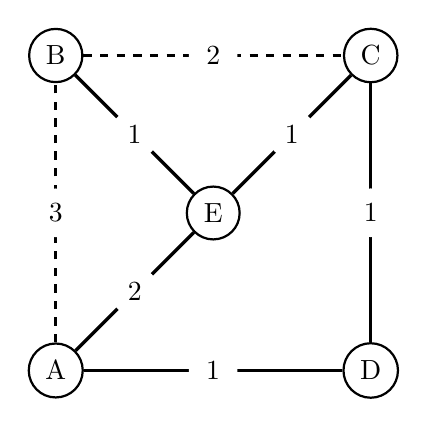
\begin{tikzpicture}
		\begin{scope}[every node/.style={circle,thick,draw}]
			\node (A) at (0,0) {A};
			\node (B) at (0,4) {B};
			\node (C) at (4,4) {C};
			\node (D) at (4,0) {D};
			\node (E) at (2,2) {E};
		\end{scope}
		
		\begin{scope}[>={Stealth[black]},
					  every node/.style={fill=white,circle},
					  every edge/.style={draw=black,very thick}]
			\path [-] (A) edge node {$2$} (E);
			\path [-] (B) edge node {$1$} (E);
			\path [-] (C) edge node {$1$} (D);
			\path [-] (E) edge node {$1$} (C);
			\path [-] (D) edge node {$1$} (A);
	
		\end{scope}
	
		\begin{scope}[>={Stealth[black]},
			every node/.style={fill=white,circle},
			every edge/.style={draw=black,very thick, dashed}]
		\path [-] (A) edge node {$3$} (B);
		\path [-] (B) edge node {$2$} (C);
	
	\end{scope}
		\end{tikzpicture}
		\caption{Contraction of node E. Shortcuts are indicated with dashed lines. After the contraction, all edges of node E can be removed.}
	\label{CH}
	\end{figure}
	

Another important aspect of CH algorithms is node ordering, which is the sorting of which nodes to contract. Optimal node ordering is proved to be an NP-hard problem \parencite{calamoneri_preprocessing_2010}. \cite{mcgeoch_contraction_2008} shows how effective node contraction does not necessitate knowing the complete order of nodes to be contracted: it can be achieved only by knowing the next node to contract. The next node to be contracted is selected using a linear combination of priority terms. The most important one is edge difference: edge difference is the number of shortcuts introduced by the contraction of a node minus the existing number of edges of that node. We want to keep this as low as possible otherwise the contracted graph will converge to the complete graph. Edge difference could be problematic as a contraction could change the edge difference of close or distant nodes, reevaluating all the graph will prove counterproductive. This issue is solved by evaluating just a neighborhood of the contracted node. Edge difference may lead to contraction happening just in a small region, this could lead to slow routing. Uniformity across the graph is thus necessary and this is achieved with heuristics, the most powerful are: Deleted Neighborhoods, Original Edges Term and Voronoi Regions \parencite{Geisberger2012}.

\section{Empirical Design}
\label{edesign}
Indexes used in the evaluation of spacial accessibility are categorized by \cite{marwal_literature_2022} in isochrones, gravity or utility based. Isochrones provide a simple and broad view of accessibility but count only the locations accessible when below a certain defined boundary. Gravity-based measures weight opportunities using a functional form of travel time or costs, they can be also integrated with features of locations such as quality of treatment for hospitals or similar. Utility-based models rely on random utility theory to evaluate locations, knowing that agents will select the ones that maximize their utility. They require low input data but still, some is necessary in order to estimate parameters of the utility function \parencite{ziemke_accessibility_2018}.

We create an index for connectivity (CI) with the main objective of ease of implementation. Thus we chose a gravity-based model with a functional form that rewards locations that are closer to a specific distance. Note that still all locations are considered when calculating the index. The connectivity index satisfies the following conditions :
	\begin{enumerate}
		\item $0<\text{CI}<1$
		\item CI depends on the minimum distance to the element of a given service (minimum distance or MD)
		\item CI depends also on the total number of elements accessible in less than a threshold distance (number of elements in neighborhood or NEN). This value is relative to the building with the most elements of a given service inside the minimum threshold distance
		\item It allows for a different weighting given to MD and NEN
		\item It gives a ``penalty'' to all those services where the closest element is more distant than fifteen minutes.
	\end{enumerate}
	We define $\boldsymbol{s}_i$ as the vector containing all distances to services in the city for building $i$. We denote $d_{min} \in \boldsymbol{s}_i: d_{min}\leq d_j \forall d_j \in  \boldsymbol{s}_i$, that is the minimum distance for service $i$ (MD). We set $\bar{d}$ as the threshold for close services. $n$ will be the number of elements in the vector where $d<\bar{d}$ (NEN). $n_{max}$ will be the maximum number of close services for any building, thus representing the best in class for a number of services inside the threshold distance. We need this measure as some services are more frequent around the city than others. Our index will be:
	\begin{equation}
		\text{CI}=\alpha f\left(d_{min}\right)+\beta \left(\frac{n}{n_{max}}\right)
	\end{equation}
	where:
	\begin{equation*}
		f(x)=
		\begin{cases} 
			1 & x\leq \bar{d} \\
			\frac{1}{x-\bar{d}+1} & x>\bar{d}
		\end{cases}
	\end{equation*}
 Note that $\alpha$ and $\beta$ must be chosen such that $\alpha+\beta=1$
 
 \begin{figure}
 	\centering
 \begin{tikzpicture}
	\begin{scope}[xshift=6cm]
		\begin{axis}[%
			title=Penality funciton for minimun distance,
			ylabel={$f(d_{min})$},
			xlabel={$d_{min}$ (s)},
			xticklabels={}
			]
			\draw [dashed] (axis cs:1,0) -- (axis cs:1,1);
			\node [left] at (axis cs:  1, 0.6) {$\bar{d}$};
			\addplot[smooth, thick,domain=\Tolerance:1-\Tolerance,samples=100]{f(x)};
			\addplot[smooth, thick,domain=1+\Tolerance:4,samples=100]{f(x)};
		\end{axis}
	\end{scope}
\end{tikzpicture}
 \end{figure}

\section{Results}
\label{res}

We created the distance matrix for each service and each public housing building as presented in section \ref{data}. In order to extract insights from those data we applied our connectivity index to the distance matrix. We chose to implement a parametrization of CI that assigned equal value to closeness ($\alpha$ parameter) and variability of services ($\beta$ parameter). This implies that $\alpha=\beta=0.5$. Another parameter that needs to be exogenously determined is $\bar{d}$, which is the threshold distance for close services. Political and academic debate on the ``15-minute city" was the main driver of parametrization choice for threshold distance of $\bar{d}=900s$ \parencite{khavarian-garmsir_15-minute_2023}. Although this threshold is deterministic, in our index it is not the only mode of evaluation, as our index is not entirely based on this value.

\subsection{Summary Statistics}

Table \ref{suumstatstab} reports summary statistics for the connectivity index of each service. We aggregate the CI calculated for each building to the service that this refers to in order to have a city-wide metric differentiated by type of service. This means, for example, that the average reported for train stations is the average CI across public housing buildings for the service of train stations.

From the average, we see that 14 services out of 22 have average CI scores of $0.5\pm0.15$. Cultural points of interest, family and addiction counseling university buildings and train stations are the services that score on average lower than this range. Cultural points obtain an exceptionally low value of $0.058004$ on average. These values could be a consequence of the tendency of cultural points of interest to be placed in the city center and thus away from the majority of public housing buildings. This view is also confirmed by the metrics described in the following paragraphs. The median provides similar insights. We see from maximum and minimum that our index ranges exactly from 1 to $0\pm0.00003$ for all services. This was indeed expected from the design of the connectivity index.

It is also interesting to see how CI scores are distributed among public housing units. For this purpose, we use skewness and kurtosis. Skewness estimates the third standardized moment of the population distribution and it is an index of the symmetry of the distribution. It ranges from $-\infty$ to $+\infty$, it is $0$ when the distribution is perfectly symmetric and takes negative or positive values based on where the asymmetry lays. Kurtosis is an estimate of the fourth standardized moment of the population distribution and it is used to compare the peakedness (weaker or heavier tails and shoulders) of a distribution to the ones of the normal. It ranges from $1$ to $\infty$ and for reference, the normal distribution has a kurtosis of $3$. Often to this metric is subtracted 3 (as in our case) to better highlight the relation with the normal distribution  \parencite{ho_descriptive_2015}. From table \ref{suumstatstab} we note that the most skewed distribution is the distance from Duomo with a value of $12.600432$. This implies that the distribution of the distance from the city center is asymmetric and the right tail extends the most. This metric shows that there is a concentration of public housing units placed close to the city center. Kurtosis is also high, implying that this metric is more has heavier tails compared to the Gaussian distribution. A concentration of data has a low value of distance from the city center but outliers are quite frequent.  Looking at the results for the CI we see that the highest value of skewness is reached by cultural points of interest. Here the interpretation differs as higher values imply better connectivity. This service has found most of the data on the lower scores of CI implying that most public housing is poorly connected with cultural points of interest. Kurtosis is also high showing that there are more outliers compared to the normal. We see that the services that come closest to having a symmetric distribution are metro stations, with a value of $0.384926$. Notably, most of the services obtain a negative value of skewness, implying that most of the scores have high values. Store and groceries seem to be the most left with a value of $-3.172366$. Looking at kurtosis 12 out of 22 services have values higher than zero and thus tails heavier than the Gaussian distribution. Postal offices, Italian schools and water fountains come very close to 0 with values of $-0.082454$, $-0.069862$ and $0.074387$ respectively.


\begin{landscape}
	\begin{table}
		\centering
		\begin{tabular}{lrrrrrrr}
			\toprule
						  Service &        Mean &      Median &    Minimum &      Maximum &    $\sigma$ &  Skewness &   Kurtosis \\
			\midrule
				  Water fountains &    0.588909 &    0.666667 &   0.000038 &     1.000000 &    0.298981 & -1.256788 &   0.074387 \\
				 Public libraries &    0.448982 &    0.666667 &   0.000035 &     1.000000 &    0.330759 & -0.545798 &  -1.568690 \\
					   Bike lanes &    0.583804 &    0.581871 &   0.000043 &     1.000000 &    0.098156 & -2.484344 &  18.249688 \\
			   Family counseling &    0.180754 &    0.000914 &   0.000032 &     1.000000 &    0.285379 &  1.013261 &  -0.832189 \\
					 Cultural POI &    0.058004 &    0.000417 &   0.000033 &     1.000000 &    0.183163 &  3.140419 &   8.898860 \\
					  News-stands &    0.579617 &    0.568966 &   0.000039 &     1.000000 &    0.094452 & -1.154315 &  15.855984 \\
					   Pharmacies &    0.614192 &    0.612903 &   0.000040 &     1.000000 &    0.125522 & -1.438254 &  10.073702 \\
				   Metro stations &    0.384926 &    0.550000 &   0.000043 &     1.000000 &    0.305534 & -0.305707 &  -1.527592 \\
					 Public parks &    0.502103 &    0.531792 &   0.000036 &     1.000000 &    0.181710 & -1.966817 &   3.413313 \\
				   Postal offices &    0.493276 &    0.562500 &   0.000039 &     1.000000 &    0.259047 & -1.147095 &  -0.082454 \\
			Addiction counseling &    0.191438 &    0.000843 &   0.000033 &     1.000000 &    0.291208 &  0.976176 &  -0.752664 \\
					 Kindergarten &    0.683411 &    0.678571 &   0.000039 &     1.000000 &    0.115460 & -2.197506 &  12.323776 \\
				  Italian schools &    0.466289 &    0.535714 &   0.000038 &     1.000000 &    0.247952 & -1.068808 &  -0.069862 \\
				 Sport facilities &    0.693574 &    0.676724 &   0.000040 &     1.000000 &    0.122241 & -1.134635 &   8.502487 \\
			   Elementary schools &    0.708579 &    0.700000 &   0.000040 &     1.000000 &    0.134471 & -1.730198 &   8.854016 \\
					 High schools &    0.422154 &    0.541667 &   0.000035 &     1.000000 &    0.281271 & -0.668483 &  -1.149812 \\
				   Middle schools &    0.608370 &    0.593023 &   0.000039 &     1.000000 &    0.135834 & -2.820057 &  11.689541 \\
				   Train stations &    0.222444 &    0.002111 &   0.000034 &     1.000000 &    0.304051 &  0.684745 &  -1.456602 \\
			 University buildings &    0.212721 &    0.001405 &   0.000037 &     1.000000 &    0.271683 &  0.630182 &  -1.281901 \\
							 wifi &    0.616373 &    0.603774 &   0.000039 &     1.000000 &    0.100988 & -1.044054 &  10.986417 \\
			 Stores and Groceries &    0.509896 &    0.515695 &   0.000038 &     1.000000 &    0.108288 & -3.172366 &  16.078387 \\
					 All services &    0.626734 &    0.613839 &   0.000043 &     1.000000 &    0.074860 &  0.992269 &  10.011883 \\
					   duomo\_dist & 5213.334094 & 4933.363499 & 318.419822 & 61032.302044 & 2533.143374 & 12.600432 & 277.884758 \\
			\bottomrule
			\end{tabular}
			
			\caption{Summary statistics on the connectivity index for each service. $\sigma$ denotes the standard deviation.}
			\label{suumstatstab}

		\end{table}	
		\end{landscape}

\subsection{Gini Index, Correlation and Mutual Information}

Table \ref{statstab} reports three statistics that further evaluate the connectivity index across services. Those are the Gini coefficient, correlation with geodesic distance from the city center and mutual information. 

The Gini coefficient adds a metric to estimate how equally the connectivity index is distributed among buildings. The Gini coefficient is calculated using the Lorenz curve, which is a polygonal line connecting points that have coordinates given by the cumulative relative frequency of a certain value and arranged increasingly. This curve is compared with the egalitarian line, that is the Lorenz curve where all variables have the same value. The index is the ratio of the area between the two curves and the area below the egalitarian line. The Gini coefficient ranges from 0 to 1. Note that the Gini coefficient is 0 when the Lorenz curve and the egalitarian line coincide, this corresponds to perfect equality. The converse is true when the Gini index is 1 \parencite{giorgi_gini_2020}. Although the Gini coefficient is often applied to income and wealth inequality, it can provide insights also when applied to the connectivity index. In this case, the value 0 will represent a perfect equality of access to a specific service among the public housing buildings. We see that the lowest Gini coefficient is achieved when considering all services across the city. This implies that overall access to services with no differentiation is quite equally distributed across public housing units. Most services perform well with nine of them under the threshold of $0.1$. Only four services performed more than $0.5$. Those are university buildings, train stations, addiction and family counseling and cultural points of interest, the worst service when it comes to equality of scores. 


We add a metric for geodesic distance in meters from the city center, that we identify with the coordinates of Duomo di Milano. Python's Geopy library allows us to calculate the geodesic distance between two points using the World Geodetic System model, the most used for this type of calculation. We also provide summary statistics for this metric and we see that on average, each public housing unit is 5968.278 meters away from the city center. The correlation column reports the Pearson correlation between each service connectivity index. We want to investigate if there is some correlation between the availability of services and the distance of the building from the city center. Notably, each service has a negative correlation between CI and distance from Duomo. This suggests that as the distance of public housing buildings from the city center increases, the availability of all services decreases. Although the previous insight is true for all services, we see a wide range of values of correlation. For example, overall services have the most negative correlation with a value of $-0.596738$. Notably for policy implications, elementary schools, middle schools and family counseling are quite negatively correlated with distance from the city center with values around $-0.4$. Public parks, public libraries, postal offices, Italian schools
and addiction counseling have correlation values of $-0.2$ and $-0.1$. Train stations and water fountains have almost no correlation with distance from the city center, implying that those services are quite diffused around the city. 

Pearson's correlation investigates linear relationships between variables. A more general measure comes from mutual information that observes also monotonic and non-monotonic relationships. We replicate the same analysis for the correlation investigating the relation between distance from the city center and connectivity index. Mutual information as described in \cite{elements} is "a measure of the amount of information that one random variable contains about another random variable". We see that the results here change substantially compared to the ones shown previously. This was expected as mutual information investigates more complex types of relations between variables. Mutual is equal to 0 when no information is provided and is maximum when the two random variables are the same. This relationship is described by the following equation
\[I(X;Y)=H(X)-H(X|Y)\]
Where $H(X)$ is Shannon's entropy of the random variable $X$ and $H(X;Y)$ the conditional entropy of $X$ and $Y$. From the previous, we get that: 
\[I(X;X)=H(X)\]
Thus in our case, the upper bound is $5.553744$, which is the mutual information of the same variable (distance from Duomo). We see that the cultural points of interest come very close to this bound, although they obtained a lower correlation. The same can be said about university buildings and all services. On the other hand, middle, elementary and Italian schools, public libraries, postal offices, kindergarten and water fountains perform the lowest value of mutual information (less than $3.000$). 

\begin{table}
\centering
\begin{tabular}{lrrr}
	\toprule
				  Service &     Gini &  Correlation &  Mutual Information \\
	\midrule
		  Water fountains & 0.240346 &    -0.053253 &            1.913922 \\
		 Public libraries & 0.367927 &    -0.193059 &            2.533260 \\
			   Bike lanes & 0.071857 &    -0.376415 &            4.534293 \\
	   Family counseling & 0.721401 &    -0.382185 &            4.458782 \\
			 Cultural POI & 0.910358 &    -0.351438 &            5.394022 \\
			  News-stands & 0.069450 &    -0.512833 &            3.071575 \\
			   Pharmacies & 0.091634 &    -0.470427 &            2.875015 \\
		   Metro stations & 0.415849 &    -0.276610 &            3.318674 \\
			 Public parks & 0.154304 &    -0.196006 &            3.898988 \\
		   Postal offices & 0.253366 &    -0.162762 &            2.340985 \\
	Addiction counseling & 0.703958 &    -0.124862 &            4.360059 \\
			 Kindergarten & 0.083242 &    -0.375858 &            2.330676 \\
		  Italian schools & 0.255305 &    -0.140015 &            2.651912 \\
		 Sport facilities & 0.089091 &    -0.280608 &            3.641130 \\
	   Elementary schools & 0.095642 &    -0.428292 &            2.814154 \\
			 High schools & 0.342531 &    -0.304161 &            3.529942 \\
		   Middle schools & 0.092428 &    -0.395775 &            2.565271 \\
		   Train stations & 0.657674 &    -0.076874 &            4.122878 \\
	 University buildings & 0.635098 &    -0.276371 &            4.844099 \\
					Public Wi-Fi & 0.079492 &    -0.478185 &            3.303520 \\
	 Stores and Groceries & 0.065545 &    -0.338781 &            3.333871 \\
			 All services & 0.057605 &    -0.596738 &            5.038962 \\
			   Distance from Duomo & 0.188589 &     1.000000 &            5.553744 \\
	\bottomrule
	\end{tabular}
	
	\caption{Statistics on the connectivity index for each service. Correlation column reports the Pearson correlation between the connectivity index and geodesic distance in meters from the city center (identified with Duomo di Milano). Gini column reports the Gini coefficient of each service. MI column reports the mutual information between the connectivity index and distance from the city center}
	\label{statstab}

\end{table}	


\begin{landscape}

	\begin{table}
    \footnotesize
	\centering
		
	

	\begin{tabular}{rrrr|rrrr|rrrr}
		\toprule
		\multicolumn{4}{l}{Family counseling} & \multicolumn{4}{l}{Addiction counseling} & \multicolumn{4}{l}{Kindergarten} \\
		  Max &   ID max &      Min &   ID min &  Max &   ID max &      Min &   ID min &      Max &   ID max &      Min &   ID min \\
		\midrule
		  1.000000 & 10004301 & 0.000155 & 20002703 &  1.000000 & 30000601 & 0.000141 & 10002701 & 1.000000 & 20000804 & 0.000941 & 10002701 \\
		  1.000000 & 51015501 & 0.000155 & 20002605 &  1.000000 & 30000504 & 0.000141 & 10003901 & 1.000000 & 51010701 & 0.000951 & 10003901 \\
		  1.000000 & 10004201 & 0.000155 & 20002606 &  1.000000 & 51016301 & 0.000158 & 41010201 & 0.964286 & 20000805 & 0.002360 & 51012601 \\
		  0.800000 & 20001102 & 0.000155 & 20002607 &  1.000000 & 30003701 & 0.000187 & 10003203 & 0.964286 & 20003501 & 0.002491 & 51016001 \\
		  0.800000 & 10003001 & 0.000155 & 20002701 &  1.000000 & 30000801 & 0.000187 & 10003204 & 0.928571 & 10003801 & 0.003155 & 30001402 \\
		  0.800000 & 10004101 & 0.000155 & 20002702 &  1.000000 & 30000701 & 0.000187 & 10002101 & 0.928571 & 10003802 & 0.004664 & 51038101 \\
		  0.800000 & 20001001 & 0.000155 & 20002801 &  1.000000 & 30003402 & 0.000195 & 10002601 & 0.928571 & 51023601 & 0.005708 & 41018505 \\
		  0.800000 & 20001101 & 0.000155 & 20002604 &  1.000000 & 30003401 & 0.000195 & 10002602 & 0.928571 & 20000801 & 0.005708 & 41018504 \\
		  0.800000 & 20001103 & 0.000155 & 20002603 &  1.000000 & 30000503 & 0.000195 & 10002604 & 0.928571 & 20000803 & 0.006098 & 41023301 \\
		  0.800000 & 20000301 & 0.000155 & 20002602 &  1.000000 & 30000502 & 0.000195 & 10002605 & 0.892857 & 51017501 & 0.535714 & 20001813 \\
		
		\end{tabular}

		\begin{tabular}{rrrr|rrrr|rrrr}
			\toprule
			\multicolumn{4}{l}{Italian schools} & \multicolumn{4}{l}{Elementary schools} & \multicolumn{4}{l}{High schools} \\
				 Max &   ID max &      Min &   ID min &    Max &   ID max &      Min &   ID min &      Max &   ID max &      Min &   ID min \\
			\midrule
			1.000000 & 30003701 & 0.000159 & 51016001 & 1.000000 & 20000801 & 0.000455 & 41021801 & 1.000000 & 10004201 & 0.000327 & 10002701 \\
			1.000000 & 30000601 & 0.000164 & 51038101 & 1.000000 & 51023601 & 0.000455 & 41021802 & 1.000000 & 10004301 & 0.000329 & 10003901 \\
			1.000000 & 30000502 & 0.000182 & 51013001 & 1.000000 & 20000201 & 0.000455 & 10003301 & 0.916667 & 20000805 & 0.000386 & 41010201 \\
			1.000000 & 30000503 & 0.000307 & 10004501 & 1.000000 & 20000804 & 0.000455 & 41021901 & 0.916667 & 51013901 & 0.000408 & 41021801 \\
			1.000000 & 30000501 & 0.000490 & 41019402 & 1.000000 & 20000805 & 0.000455 & 41021902 & 0.916667 & 20000804 & 0.000408 & 10003301 \\
			1.000000 & 30000504 & 0.000490 & 41019401 & 1.000000 & 51010701 & 0.001782 & 30001402 & 0.916667 & 20000201 & 0.000408 & 41021901 \\
			0.964286 & 20000401 & 0.000519 & 51023702 & 0.987500 & 10003802 & 0.002147 & 51016001 & 0.916667 & 20000801 & 0.000408 & 41021802 \\
			0.928571 & 20000101 & 0.000519 & 51023701 & 0.987500 & 51014901 & 0.002849 & 51012601 & 0.916667 & 20000802 & 0.000408 & 41021902 \\
			0.928571 & 20000102 & 0.000519 & 51023703 & 0.987500 & 41019101 & 0.003587 & 51038101 & 0.916667 & 20000803 & 0.000448 & 41018505 \\
			0.928571 & 20000103 & 0.000526 & 51023705 & 0.987500 & 41019102 & 0.003922 & 41018801 & 0.916667 & 51010701 & 0.000448 & 41018504 \\
			
			\end{tabular}

			\begin{tabular}{rrrr|rrrr|rrrr}
				\toprule
				\multicolumn{4}{l}{Middle schools} & \multicolumn{4}{l}{Stores and Groceries} & \multicolumn{4}{l}{All services} \\
					 Max &   ID max &      Min &   ID min &      Max &   ID max &      Min &   ID min &      Max &   ID max &      Min &   ID min \\
				\midrule
				1.000000 & 41019802 & 0.000354 & 41021801 & 1.000000 & 10004301 & 0.000547 & 41021902 & 1.000000 & 10004301 & 0.502790 & 41021901 \\
				1.000000 & 10004301 & 0.000354 & 10003301 & 0.986547 & 10004201 & 0.000547 & 41021801 & 0.980469 & 20000401 & 0.502790 & 41021902 \\
				1.000000 & 41019801 & 0.000354 & 41021802 & 0.919283 & 20000401 & 0.000547 & 41021802 & 0.974330 & 10004201 & 0.502790 & 41021802 \\
				0.906977 & 10004201 & 0.000354 & 41021901 & 0.883408 & 30000601 & 0.000547 & 41021901 & 0.952567 & 20000201 & 0.502790 & 41021801 \\
				0.906977 & 10001801 & 0.000354 & 41021902 & 0.831839 & 30003701 & 0.000547 & 10003301 & 0.938058 & 20001001 & 0.502790 & 10003301 \\
				0.872093 & 51015501 & 0.000473 & 51016001 & 0.820628 & 20001001 & 0.000573 & 10002701 & 0.921875 & 20000101 & 0.504464 & 30001402 \\
				0.825581 & 20000802 & 0.000518 & 51038101 & 0.784753 & 30000501 & 0.000577 & 10003901 & 0.920201 & 20000103 & 0.506138 & 51016001 \\
				0.825581 & 51013801 & 0.000668 & 41019602 & 0.748879 & 30000502 & 0.000743 & 30001402 & 0.914062 & 20000102 & 0.507254 & 51038101 \\
				0.825581 & 20003801 & 0.000668 & 51017101 & 0.748879 & 30000504 & 0.001018 & 51012601 & 0.904576 & 30000601 & 0.515067 & 10002701 \\
				0.825581 & 51010801 & 0.000668 & 51017103 & 0.733184 & 30000503 & 0.002304 & 30001901 & 0.901786 & 51013801 & 0.515625 & 10003901 \\
				\bottomrule
				\end{tabular}
	\caption{best and worst performers for a selection of services. Max (Min) reports the top (bottom) 10 scores and ID max (min) the associated ID of the housing buildings associated with the score}
	\label{minmax}
	\end{table}		
			
				
\end{landscape}

\subsection{Best and Worst Performers}

Table \ref{minmax} reports the best and worst performers in a selection of the services analyzed. We note that the public housing building 10004301 scores the best connectivity index in Family counseling, Stores and Groceries and overall services with all scores of 1. Notably, it also scores second for high schools and middle schools connectivity. This public housing building is located in Via Bergamini 1, the most central unit in our dataset with a geodesic distance from Duomo of 318.4 $m$. Build between the XVIII and XIX centuries, it was acquired by the city of Milan with an esproprio con determinazione amichevole dell’indennità (expropriation with compensation that was agreed upon) on the third of February 1938. In this building, the real estate registry indicates that there should be 51 apartments \parencite{breda_tua_2016}.

Unit 10002701 on the other hand, is the worst performer in Addiction counseling, kindergarten and high schools connectivity with scores of 0.000141, 0.000941 and 0.000327 respectively. It also scores in the worst ten units for groceries and stores and overall services. This unit is located in Via Guido Ucelli di Nemi 58, in the Ponte Lambro district, at the city limits. It was built in 1956 with the style of Case Minime (minimal hoses) that were built with common structures and materials.  Building 10002901, Via San Mamete 8, is the first one to be built according to those standards, in total there are 25 examples of this type of building around the city. In Uccelli di Nemi 58 there are 35 apartments of 40 $m^2$ with one or two rooms. The ceiling height is 2.8 meters. It was poorly maintained and until 2008, was a renewal program of the Comune di Milano that included also other buildings in this district completely renovated this building, with the objective of increasing the capacity of users of 20\% \parencite{breda_tua_2016}.

Unit 41021801 has the lowest connectivity for elementary (0.000455) and middle school (0.000354). It is also in the worst 10 for connectivity with stores and groceries and high schools. It is also the fourth worst performer for overall connectivity with a score of 0.502790. This building is located in Via San Bernardo 48, close to the Abbazia of Chiaravalle, in the agricultural countryside at the southern city limits \parencite{breda_tua_2016}. Built in 1985,  this building was renovated in recent years using EU-GUGLE founds \footnote{European Cities Serving as Green Urban Gate Towards Leadership in Sustainable Energy}. This project was an experiment to demonstrate the feasibility of net zero districts in different urban areas across the Union. Practices implemented across cities will be useful to implement similar objectives in other cities. Vienna (Austria), Aachen (Germany), Milan (Italy), Sestao (Spain), Tampere (Finland) and Bratislava (Slovakia) obtained a total of  € 16,785,372 for the renovation of 226,000 $m^2$. Specifically for Via San Bernardo 48, the building undergone an envelope retrofitting, installation of heat recovery on exhaust air, photovoltaic and energy management systems. Additional renovations were made at the district level with the installation of a bike path connecting with the city center (planned but not yet constructed) and renovations made to the district's kindergarten \parencite{neri_slow_2020}. Other buildings obtained the EU-GUGLE founds, namely via Feltrinelli 11 and 16 (41039901) and via San Bernardo 50 \parencite{morishita2017eu}.

The worst performers of overall services are buildings 41021901 and 41021902, both located in via San Bernardo 29/A, very close to the previously covered via San Bernardo 48. These buildings obtained an identical score of 0.502790, and performed poorly also in connectivity to schools and stores and groceries. Similarly to  via San Bernardo 48, they also received another European found named Sharing Cities. This fund allocated 500 million euros to  Bordeaux (France), Burgas (Bulgaria), Lisbon (Portugal), London (the United Kingdom), Milan (Italy), and Warsaw (Poland). Milan used the funds to implement building retrofit, improve shared e-mobility, install sustainable energy management systems and smart lamp posts. Funds were allocated using co-design principles, involving all stakeholders of the districts that were affected.

Additional qualitative insights can be drawn from maps that report the connectivity index scores of units across the city. Those reported in appendix \ref{maps}. We note that services such as kindergarten, elementary and middle schools and all services have connectivity scores that gradually decrease when the distance from the city center increases. On the contrary, we see other services that seem to be targeted to the city periphery, such as addiction and family counseling, that are both highly connected with specific sectors of the city that do not overlap with the city center.

\section{Conclusion}
\label{conclusion}

This analysis was intended as an explorative study of public housing and accessibility to fundamental services across the city of Milan. The main focus was not on causal relations but on building a methodology to easily obtain distances and evaluate them using an index. Future developments are possible, first of all by moving towards causality. Also adding adding more cities to the analysis could prove interesting in order to compare accessibility across different municipalities. Although the principal objective of the connectivity index is to be easily interpretable, more insights can be drawn by changing methodology in the evaluation of distances, mainly by applying random utility models. Said so the most interesting insights may be drawn from the analysis of the relation between additional data not included in our datasets: accessibility to schools and the impact on grades, health rates and accessibility to sports facilities and accessibility to parks. 

The advantage of our methodology is that it is an easy to implement and open-source alternative with similar functionalities to more expensive private tools. This allows for funding to be directed towards different data sources. The code used in this paper is also published in Github in order for future research to build on what has already been achieved here. Interesting improvements in the code may integrate public transport as a mode of transportation, which is implementable but tricky as highly time-dependent. Another factor that could be included is traffic, especially important for the analysis of cities where cars are still the dominant transport type. 

We showed how there exists a high correlation between distance from the city center and connectivity to different services. This correlation is explored with different statistical methods. We also looked at the distributional differences in accessibility between public housing units and interestingly we found that accessibility is quite equally distributed.  

All this information is important for two reasons: firstly by identifying areas of intervention, such as the southern agricultural periphery, that has units with the lowest scores. Another important aspect is to highlight best in class, that may have the best returns for the families that inhabit those units. Knowing all of this will be an important factor in the allocation of funding that is limited. 

Public housing is important as it can be seen not only as a policy tool that allows the poorest to obtain affordable housing. Additionally, it may provide them with access to fundamental services that will never be available to them without public support. Public housing thus could ideally become a social elevator that brings in vulnerable families and provides them with better services and schooling that was previously impossible. This research question is thus not only a question of standards of life for the current generation that obtains public housing but also how this service could provide a social ladder to those who access it.  Is thus important to understand how this accessibility is spread around the city and the relation it has with common policy outcomes such as a decrease in educational and wealth inequality, improvement of standards of life and access to services.  


\newpage
\printbibliography

\newpage

\appendix

\section{Maps}
\label{maps}

This section shows two different types of maps: figure \ref{servicemap} shows all services that were extracted from the Open data portal of Comune di Milano. Figure \ref{cimap} plots the locations of the social housing buildings owned by Comune di Milano and the associated connectivity index for that specific service.

\begin{figure}[h!]
	\includegraphics[width=\textwidth]{services_map.pdf}
	\caption{Map of the city of Milan showing all services used for the analysis}
	\label{servicemap}
\end{figure}

\newpage

\begin{figure}[h!]
	\includegraphics[width=0.32\textwidth]{sinf.pdf}\hfill
	\includegraphics[width=0.32\textwidth]{sprim.pdf}\hfill
	\includegraphics[width=0.32\textwidth]{ssec.pdf}
	\\[\smallskipamount]
	\includegraphics[width=0.32\textwidth]{ss2.pdf}\hfill
	\includegraphics[width=0.32\textwidth]{sita.pdf}\hfill
	\includegraphics[width=0.32\textwidth]{cult.pdf}
	\\[\smallskipamount]
	\includegraphics[width=0.32\textwidth]{metro.pdf}\hfill
	\includegraphics[width=0.32\textwidth]{serd.pdf}\hfill
	\includegraphics[width=0.32\textwidth]{consu.pdf}
	\\[\smallskipamount]
	\includegraphics[width=0.32\textwidth]{distr.pdf}\hfill
	\includegraphics[width=0.32\textwidth]{parchi.pdf}\hfill
	\includegraphics[width=0.32\textwidth]{all.pdf}
	\caption{Plots of connectivity index for a selection of the services analyzed. Each dot corresponds to one public housing building}
	\label{cimap}
\end{figure}



\section{Code overview}
\label{code}

In this section, we will cover how to run OSRM backend locally on a PC and interact with it in Python \footnote{We build on information from the readme of OSRM backend and Michael Yan’s guide \url{https://www.thinkdatascience.com/post/2020-03-03-osrm/osrm/}}. We will demonstrate the process of running it on Windows with WSL installed, but the process is similar to other operating systems. Other than WSL is also necessary to have installed Docker Desktop. This is necessary because OSRM is installed as a docker image, thus removing any OS compatibility problem that may arise.

First of all, start a WSL session and navigate to your directory. In this example the directory folder is called "dir" and the user is "myuser"
\begin{lstlisting}[language=bash]
cd "/mnt/c/users/myuser/dir/"
\end{lstlisting}

Now we need to download the Open Street Map of the desired area. We will use the Geofabrik service (that can be called directly from the command line). Here we will demonstrate an example using the Nord ovest area of Italy, but a section of all the world can be downloaded. 
\begin{lstlisting}[language=bash, breaklines=true]
wget http://download.geofabrik.de/europe/italy/nord-ovest-latest.osm.pbf
\end{lstlisting}
Note that if the resources of the PC are limited, especially RAM, a larger area may prove impossible to run on OSRM. An alternative is to select a smaller area on Geofabrik or to manually process the OSM file using Osmconvert. 

Now we move to the actual computational part. We are preprocessing the map downloaded above. Note that this is transportation type specific: here we are running the preprocessing part with a foot.lua profile. If you want to change to a car or bike transportation type you will have to change this part with either car.lua or bike.lua. Subsequent changes of transportation profiles will need a new preprocessing.
\begin{lstlisting}[language=bash, breaklines=true]
docker run -t -v "${PWD}:/data" ghcr.io/project-osrm/osrm-backend osrm-extract -p /opt/foot.lua /data/nord-ovest-latest.osm.pbf || "osrm-extract failed"
\end{lstlisting}
By running the command above docker will realize that the OSRM image is not installed, by showing the following output:
\begin{lstlisting}[language=bash, breaklines=true]
Unable to find image 'ghcr.io/project-osrm/osrm-backend:latest' locally
latest: Pulling from project-osrm/osrm-backend
\end{lstlisting}
This will trigger an automatic pull from the latest version if docker is correctly installed on your PC.

The following commands start the OSRM local version with a     Multi-Level Dijkstra (MLD) algorithm.
\begin{lstlisting}[language=bash, breaklines=true]
docker run -t -v "${PWD}:/data" ghcr.io/project-osrm/osrm-backend osrm-partition /data/nord-ovest-latest.osrm || "osrm-partition failed"

docker run -t -v "${PWD}:/data" ghcr.io/project-osrm/osrm-backend osrm-customize /data/nord-ovest-latest.osrm || "osrm-customize failed"

docker run -t -i -p 5000:5000 -v "${PWD}:/data" ghcr.io/project-osrm/osrm-backend osrm-routed --algorithm mld /data/nord-ovest-latest.osrm
\end{lstlisting}

Alternatively to run OSRM with Contraction Hierarchies (CH) run the following code must be used instead:
\begin{lstlisting}[language=bash, breaklines=true]
docker run -t -v "${PWD}:/data" ghcr.io/project-osrm/osrm-backend osrm-contract /data/nord-ovest-latest.osrm || "osrm-partition failed"
	
docker run -t -i -p 5000:5000 -v "${PWD}:/data" ghcr.io/project-osrm/osrm-backend osrm-routed --algorithm ch /data/nord-ovest-latest.osrm
\end{lstlisting}
The process above needs to run only the first time or when you want to change the transportation mode, algorithm or area of routing. The only command that needs to run every time is the last one.

After all of this, we can make a simple request of routing to test that everything runs.
\begin{lstlisting}[language=bash, breaklines=true]
curl "http://127.0.0.1:5000/route/v1/driving/13.388860,52.517037;13.385983,52.496891?steps=true"
\end{lstlisting}

To interact with OSRM in Python we use the following code\footnote{Full code available on the Github repository}:
\begin{lstlisting}[language=python, breaklines=true]
import requests

def get_route(pickup_lon, pickup_lat, dropoff_lon, dropoff_lat):
    loc = "{},{};{},{}".format(pickup_lon, pickup_lat, dropoff_lon, dropoff_lat)
    url = "http://127.0.0.1:5000/route/v1/driving/"
    r = requests.get(url + loc)
    if r.status_code!= 200:
        return {}

    res = r.json()
    duration = res['routes'][0]['duration']
    distance = res['routes'][0]['distance']

    return duration

get_route(9.1930893, 45.5053767	,9.23444555, 45.49610165)
\end{lstlisting}








\end{document}